\documentclass{sig-alternate-05-2015}

%\usepackage[ruled]{algorithm2e}
%\renewcommand{\algorithmcfname}{ALGORITHM}
%\usepackage{amsmath,amsfonts,amssymb,bbm} 
%\usepackage[numbers,sort&compress]{natbib} % for citet
%\SetArgSty{textrm}  % for algorithm2e
%\SetAlFnt{\small}
%\SetAlCapFnt{\small}
%\SetAlCapNameFnt{\small}
%\SetAlCapHSkip{0pt}

\usepackage[utf8]{inputenc}
\usepackage{afterpage}
\usepackage{tikz}
\usetikzlibrary{arrows,chains,decorations.pathreplacing}
%\usepackage{draftwatermark}
%\SetWatermarkText{DRAFT}
\newcommand{\beq}{\begin{eqnarray}}
\newcommand{\eeq}{\end{eqnarray}}
\DeclareMathOperator{\wbf}{wBF}
\newtheorem{theorem}{Theorem}

\begin{document}

% Copyright
\setcopyright{acmcopyright}
%\setcopyright{acmlicensed}
%\setcopyright{rightsretained}
%\setcopyright{usgov}
%\setcopyright{usgovmixed}
%\setcopyright{cagov}
%\setcopyright{cagovmixed}


% DOI
%\doi{10.475/123_4}

% ISBN
%\isbn{123-4567-24-567/08/06}

%Conference
\conferenceinfo{WSDM '17}{February 6--10, 2017, Cambridge, UK, USA}

\acmPrice{\$15.00}

%
% --- Author Metadata here ---
%\conferenceinfo{WOODSTOCK}{'97 El Paso, Texas USA}
%\CopyrightYear{2007} % Allows default copyright year (20XX) to be over-ridden - IF NEED BE.
%\crdata{0-12345-67-8/90/01}  % Allows default copyright data (0-89791-88-6/97/05) to be over-ridden - IF NEED BE.
% --- End of Author Metadata ---

\title{Attack-Tolerant Networks: A Structural, Multipath Approach}
%
% You need the command \numberofauthors to handle the 'placement
% and alignment' of the authors beneath the title.
%
% For aesthetic reasons, we recommend 'three authors at a time'
% i.e. three 'name/affiliation blocks' be placed beneath the title.
%
% NOTE: You are NOT restricted in how many 'rows' of
% "name/affiliations" may appear. We just ask that you restrict
% the number of 'columns' to three.
%
% Because of the available 'opening page real-estate'
% we ask you to refrain from putting more than six authors
% (two rows with three columns) beneath the article title.
% More than six makes the first-page appear very cluttered indeed.
%
% Use the \alignauthor commands to handle the names
% and affiliations for an 'aesthetic maximum' of six authors.
% Add names, affiliations, addresses for
% the seventh etc. author(s) as the argument for the
% \additionalauthors command.
% These 'additional authors' will be output/set for you
% without further effort on your part as the last section in
% the body of your article BEFORE References or any Appendices.

\numberofauthors{1} %  in this sample file, there are a *total*
% of EIGHT authors. SIX appear on the 'first-page' (for formatting
% reasons) and the remaining two appear in the \additionalauthors section.
%
\author{
% You can go ahead and credit any number of authors here,
% e.g. one 'row of three' or two rows (consisting of one row of three
% and a second row of one, two or three).
%
% The command \alignauthor (no curly braces needed) should
% precede each author name, affiliation/snail-mail address and
% e-mail address. Additionally, tag each line of
% affiliation/address with \affaddr, and tag the
% e-mail address with \email.
%
% 1st. author
\alignauthor
Anonymized Authors
}
%       \affaddr{Institute for Clarity in Documentation}\\
%       \affaddr{1932 Wallamaloo Lane}\\
%       \affaddr{Wallamaloo, New Zealand}\\
%       \email{trovato@corporation.com}
% 2nd. author
%\alignauthor
%G.K.M. Tobin\titlenote{The secretary disavows
%any knowledge of this author's actions.}\\
%       \affaddr{Institute for Clarity in Documentation}\\
%       \affaddr{P.O. Box 1212}\\
%       \affaddr{Dublin, Ohio 43017-6221}\\
%       \email{webmaster@marysville-ohio.com}
% 3rd. author

\maketitle
\begin{abstract}
Networks with single points of failure are particularly susceptible to
adversarial faults, in which an attacker targets nodes strategically.
In communication networks, these types of attacks leave users vulnerable to
censorship and targeted surveillance.
Centralized networks have single points of failure by definition,
leading to a growing popularity in decentralized architectures and protocols.
However, centralized network structure can arise even when protocols are
decentralized.
While based on decentralized protocols, the Internet and World-Wide Web have
been shown both theoretically and historically to be highly susceptible to
adversarial faults, in part due to emergent, structural centralization.
Existing network trust models, such as webs of trust, fail to adequately address
network structure. We develop a partial trust model that incorporates network
structure and which makes weaker, more realistic transitivity assumptions than
webs of trust. We show that the partial trust model, when combined with
concurrent multipath routing, allows standard fault tolerance techniques to be
applied to communication across complex networks. We also provide a specific
routing algorithm for implementing this scheme on the butterfly network
topology.
When network topology can be dictated, these results can be used to create
scalable, attack-tolerant infrastructures. More generally, our results provide
a formalism for evaluating the effects of network structure on adversarial
fault tolerance.
\end{abstract}


%
% The code below should be generated by the tool at
% http://dl.acm.org/ccs.cfm
% Please copy and paste the code instead of the example below. 
%
\begin{CCSXML}
<ccs2012>
<concept>
<concept_id>10002978.10002986</concept_id>
<concept_desc>Security and privacy~Formal methods and theory of security</concept_desc>
<concept_significance>500</concept_significance>
</concept>
<concept>
<concept_id>10003033.10003034</concept_id>
<concept_desc>Networks~Network architectures</concept_desc>
<concept_significance>500</concept_significance>
</concept>
<concept>
<concept_id>10011007.10010940.10010971.10010972.10010540</concept_id>
<concept_desc>Software and its engineering~Peer-to-peer architectures</concept_desc>
<concept_significance>500</concept_significance>
</concept>
</ccs2012>
\end{CCSXML} 

\ccsdesc[500]{Security and privacy~Formal methods and theory of security}
\ccsdesc[500]{Networks~Network architectures}
\ccsdesc[500]{Software and its engineering~Peer-to-peer architectures}

%
% End generated code
%

%
%  Use this command to print the description
%
\printccsdesc

% We no longer use \terms command
%\terms{Theory}

\keywords{networks; decentralization; fault tolerance; routing; multipath routing; adversarial faults; information security}

\section{Introduction}

Large-scale communication networks, exemplified by the Internet,
have become ubiquitous, and are now crucial infrastructure for
individuals, communities, and organizations around the world.
As with any critical infrastructure, the cost of a failure can be
immense, so methods for tolerating various kind of faults are an
important and ongoing area of research
\cite{zin_survey_2015,albert_error_2000,sterbenz_resilience_2010}.
In fact, the decentralized design of the Internet was intended to protect
against targeted attacks, such as nuclear strikes
\cite{baran_distributed_1964}.
Such targeted attacks are formally described as {\em adversarial faults}
and are some of the most difficult to protect against.
Both theoretical results and recent events (described below)
have demonstrated that
the Internet is surprisingly vulnerable to adversarial faults.
Decentralization remains a promising approach to building resilient networks,
but further work is needed to understand the relationship between
decentralized network structure and adversarial fault tolerance.

Analysis of the Internet's router network has shown that while it is remarkably
resilient against random faults,
it is highly susceptible to adversarial faults \cite{albert_error_2000}.
These results have been attributed to the scale-free structure of the Internet's
router network
\cite{barabasi_emergence_1999,barabasi_scale-free_2009}.
In scale-free networks and other networks with heavy-tail degree distributions,
random failures are highly likely to pick low-degree nodes, thus having
little effect,
while adversarial faults target the small number of high-degree nodes,
thus removing a large number of edges with each fault.
So while the {\em protocols} of the Internet are decentralized,
the {\em network structure} is somewhat centralized. 
In other words, the protocols of the Internet do not {\em require}
centralization, but centralization may still emerge from the sociotechnical
processes that create its network structure.

The Internet's vulnerability to censorship and other targeted attacks
has been confirmed by the success of several such attacks.
For example, in 2008, YouTube suffered a worldwide outage for several hours
when a service provider in Pakistan advertised false routing information
\cite{hunter_pakistan_2008}.
The action (known as a {\em black hole attack}) was intended to censor YouTube
within Pakistan only, but resulted in a worldwide cascading failure.
Such vulnerabilities are not limited to any one system or protocol,
but result from the network structure itself.
With strong theoretical and historical evidence that network structure
can create vulnerabilities,
methods for analyzing structural vulnerabilities and for designing
fault tolerant networks are needed.
This paper presents several contributions towards advancing those goals.

We consider a setting in which a source node (Alice)
in a network attempts to route a message
to a target node (Bob) by forwarding it through the links of the network.
We assume that some nodes in the network may be compromised by an attacker
(Mal).
We assume that Mal has full knowledge of the network structure, but has
limited resources and thus can only compromise a fixed number of nodes.
Compromised nodes may behave incorrectly by blocking the message,
changing the message content, or routing the message incorrectly.
In order to evaluate network-based techniques for mitigating such attacks,
we develop a {\em partial trust} model,
similar to the commonly used web of trust approach
\cite{zimmermann_official_1995,ferguson_practical_2003},
but making weaker (more realistic) assumptions of trust transitivity,
and incorporating network structure.
The partial trust model can be used to design and analyze communication
schemes that tolerate adversarial faults,
even when no single path through the network is fully trusted.

Using the partial trust model, we are able to model the nodes in complex
networks as being directly linked to each other by a number of
redundant channels.
This models enables the application of standard error detection techniques
\cite{avizienis_basic_2004, von_neumann_probabilistic_1956},
which rely on independent errors.
While adversarial faults along a single path are correlated,
faults in independent paths are not.
Thus fault tolerance techniques can be applied,
even in the presence of adversarial errors,
when messages are sent in parallel,
a technique known as {\em concurrent multipath routing}
\cite{zin_survey_2015, qadir_exploiting_2015, khiani_comparative_2013}.
The receiver can then use the redundant messages to detect and/or correct
errors.
Using the partial trust model, we formally evaluate the 
effects of network structure on attack-resistance and show that the probability
of undetected errors decreases exponentially with the number of
independent paths between source and destination,
even when no individual path is entirely trusted.

Our specific multipath fault tolerance scheme relies on the existence
and discoverability of multiple redundant paths between the source and
the destination.
Implementation thus requires a routing algorithm.
While not a requirement, this technique is well-suited for
{\em structured networks},
in which links between nodes are constrained to a particular architecture.

In particular, we provide a novel concurrent multipath routing algorithm
on the butterfly network topology and use the partial trust model to prove
a high level of adversarial fault tolerance.
The butterfly topology is popular in parallel processing
\cite{kshemkalyani_distributed_2008} and
peer-to-peer \cite{lua_survey_2005, korzun_structured_2013}
applications, due to its regular structure and high connectivity.
While the ability to control network topology is only achievable in some
applications, those applications are nonetheless significant,
e.g. overlay networks \cite{lua_survey_2005, korzun_structured_2013},
formal organizations \cite{mohr_explaining_1982},
government-regulated cellular networks \cite{walker_mass_2012},
and call tree notification systems \cite{nickerson_thinking_2010}.

Our main contributions are:
\begin{itemize}
\item{We develop a decentralized {\em partial trust model},
which makes weaker transitivity assumptions than web-of-trust models,
and makes it possible to analyze the effect of network structure on
adversarial fault tolerance;}
\item{We show that the partial trust model enables standard fault
tolerance techniques to be applied to adversarial faults in
complex communication networks.
We find that the probability of detecting adversarial faults
approaches 1 exponentially as the number of independent paths between
sender and receiver increases;}
\item{We present a scalable, efficient, and attack-tolerant concurrent
multipath routing algorithm on the butterfly network topology.}
\end{itemize}

This paper is organized as follows.
Section 2. reviews background and related work.
Section 3. discusses the desired properties of attack-tolerant network
infrastructure.
Section 4. describes the partial trust model.
Section 5. describes a general technique for multipath fault tolerance on
structured networks.
Section 6. describes a routing algorithm for multipath fault tolerance
on the butterfly network topology.
Section 7. discusses the our results.
And Section 8. concludes.

\section{Background and Related Work}

Many distributed consensus protocols (such as those used by cryptocurrencies)
are designed to provide tolerance against arbitrary or adversarial faults.
Byzantine agreement protocols
\cite{lamport_byzantine_1982,castro_practical_1999}
provide tolerance against arbitrary faults (including attacks) under
some circumstances, but are limited to small networks due to poor scalability.
Proof-of-work \cite{dwork_pricing_1993,nakamoto_bitcoin:_2008}
and proof-of-stake \cite{king_ppcoin:_2012}
provide better scalability,
but are wasteful of computational and energy resources.
Federated Byzantine Agreement (FBA) \cite{mazieres_stellar_2015}
is scalable, allows for flexible trust,
and optimal fault tolerance for a given network (under its assumptions).
However, FBA does not provide a method for evaluating the
fault tolerance properties of different network structures
or calculating how the failure probability for a particular network.
The multipath fault tolerance scheme we propose is the
first example we're aware of that allows adversarial fault tolerance
to be quantified as a function of network structure.

Most existing adversarial fault tolerance schemes focus on end-to-end,
protocol-based, cryptographic solutions
\cite{ferguson_practical_2003}.
A fully decentralized architecture must be decentralized both in protocol and
in network structure.
There are however, a few notable fault tolerance schemes
that focus on network structure.
Fiat and Saia described a scheme that combines the butterfly topology
with expander graphs to create a highly censorship-resistant content-addressable
network \cite{fiat_censorship_2002},
although this scheme exhibits poor scaling due to a very high level of data
replication.
Perhaps the most mature structural solution is the Freenet collaboration
\cite{clarke_freenet:_2001}.
Freenet uses secret sharing
\cite{shamir_how_1979, blakley_safeguarding_1979}
and small-world routing
\cite{zhang_using_2002,kleinberg_small-world_2000}
to create a content-addressable network with a high level of both
confidentiality and censorship resistance.
Freenet guarantees that data is stored redundantly,
but still allows for centralized network structure and thus single points
of failure as data travels from its origin to the redundant storage locations.

{\em Multipath routing} protocols send redundant information
over multiple paths when routing a message through a network,
in contrast to traditional {\em unipath} routing, which uses
a single path.
Multipath routing can have many benefits, including reduced congestion,
increased throughput, and more reliability
\cite{qadir_exploiting_2015}.
Many of these routing protocols offer increased confidentiality
\cite{zin_survey_2015}.
Some approaches utilize redundant paths as backups for increased
fault tolerance
\cite{alrajeh_secure_2013},
and some specifically protect against adversarial faults
\cite{kohno_improvement_2012, khalil_unmask:_2010, lou_h-spread:_2006}.
Most work on multipath routing has been motivated by applications related to
wireless sensor networks (WSNs),
and have thus focused on ad hoc, unstructured networks, often having a central
base station.
The partial trust model presented in this paper provides a more general
way to evaluate the effect of network structure on adversarial fault tolerance.
The method of Liu et al.
\cite{liu_secure_2012}
routes multiple messages first to random peers and then
to their final destination.
The butterfly routing algorithm we present takes a conceptually similar
approach,
routing from the source to several intermediaries, and then to the destination.

Our proposed routing algorithm makes use of a
{\em structured network}, in which link structure is predetermined.
Such networks can be designed to have favorable structural and routing
properties,
at the expense of complicating the addition or removal of nodes.
Structured networks have been a popular tool in parallel processing
architectures \cite{kshemkalyani_distributed_2008}.
More recently, peer-to-peer systems based on distributed hash tables have used
structured ``overlay'' networks to map table keys to local TCP/IP routes
\cite{lua_survey_2005,korzun_structured_2013}.

\section{Attack-Tolerant Infrastructure}

In this section, we describe the functional properties required of an
attack-tolerant network,
which serve as guiding principles in later sections.
We pay special attention to a property we call
{\em stabilizing asymmetry}.

\subsection{Functional Properties}

\begin{description}
\item[Scalability:]
For large scale networks it is important that the infrastructure allows
for the network to grow while remaining functional.
In practice, people, devices, and connections, have limited capabilities
and these limitations need to be considered as part of the design of the
infrastructure. 

\item [Decentralization:]
Systems having single points of failure are less tolerant against faults at
those points.
The existence of such points not only increases the likelihood that an attack
will succeed,
but also incentivizes attack by presenting effective targets.
In order to minimize single points of failure,
attack tolerant infrastructures must use decentralized protocols and
decentralized network structures.

\item[Stabilizing asymmetry:]
In the context of international conflict,
{\em asymmetric conflicts} are a special case that makes it possible for the
less powerful party to have an advantage over the more powerful party
\cite{mack_why_1975}.
In asymmetric conflicts, the same level of resource expenditure yields different
results for different parties;
the attacker's resources are either more or less effective than the defender's.
We call the latter case stabilizing asymmetry,
because it lowers the incentive to attack.
With this in mind, an attack-resistant infrastructure will benefit from a high
level of stabilizing asymmetry.

\end{description}
\subsection{Structural Properties}

We are specifically concerned with network structure-based approaches to
fault tolerance.
In networks, specific structural properties are required to achieve the
functional properties described above.
\begin{description}
\item [Sparsity and low diameter:]
To achieve scalability, networks must be {\em sparse} and have a
{\em low diameter}.
In practical settings, humans and devices have an upper limit on the number
of connections they can maintain (e.g., Dunbar's number
\cite{dunbar_neocortex_1992}).
In sparse networks, the number of links grows slowly as the network grows in
size, allowing the network to scale without exceeding the nodes' capacity for
links.
Similarly, low-diameter guarantees that as a network grows, a short path will
still exist between any pair of nodes.
While low diameter guarantees a path exists,
paths are only useful if an efficient {\em routing} algorithm exists
to find them.

\item [Uniform centrality:]
There are many ways to measure node centrality in networks
\cite{freeman_centrality_1978}.
The more uniform these measures are across nodes, the more decentralized
a network is.
Centrality is minimized in {\em vertex transitive} networks,
for which an edge-preserving map
always exists from any node to any other node.
In other words, all nodes occupy structurally indistinguishable positions
in the network.

\item [Redundancy:]
In a network, redundancy refers to the existence of multiple non-overlapping
paths between nodes or components.
Redundancy can help reduce single points of failure and decrease
centralization.
One measure of redundancy is given by the ratio of edges to nodes
\cite{baran_distributed_1964}.
A single point of failure occurs when a node holds a uniquely
central position.
When alternative paths are added to bypass central nodes,
the network becomes more redundant.

\end{description}

\section{Trust and Fault Tolerance}

The requirement that networks remain sparse has important implications for
resilience.
As such networks grow, the number of nodes will exceed the number of links
any single node can support.
As a result, some pairs of nodes are only connected indirectly,
through at least one intermediary node.
These intermediary nodes are targets for potential attacks,
making network paths potentially unreliable.

Within the field of {\em fault tolerance},
many techniques have been developed for building reliable systems
out of unreliable components
\cite{avizienis_basic_2004, von_neumann_probabilistic_1956}.
We will make use of standard fault tolerance terminology, summarized here.
A {\em fault} occurs when one component
of a system behaves incorrectly (e.g., a routing node blocking or
altering a message).
The result of that fault (e.g., a recipient receiving conflicting messages)
is an {\em error} state.
If the error is undetected or corrected to the wrong value, the system is
said to have experienced a {\em failure} (e.g., an altered message is
accepted as authentic).
We are concerned in particular with {\em adversarial faults},
which (as opposed to random faults)
are chosen strategically to maximize the likelihood of a failure.

In communication networks, 
the threat model is as follows: Alice sends a message to
Bob via one or more intermediaries,
but some intermediaries may block, change, or re-route the message.
The ability to tolerate these types of adversarial attacks depends on
Alice and Bob's ability to either find a path they {\em trust},
or to communicate successfully across untrusted paths.

Both centralized and decentralized approaches are commonly used to create
trust infrastructures.
Centralized approaches such as {\em public key infrastructure} (PKI)
suffer from a number of vulnerabilities
\cite{ellison_ten_2000},
which stem largely from the single points of failure inherent to
centralization.

The well-known and widely-used {\em web of trust} model
\cite{zimmermann_official_1995,ferguson_practical_2003}
is a decentralized alternative.
In a web of trust,
individuals choose who they trust initially.
Trust is then extended to new individuals if they are vouched for by a
currently-trusted individual,
making it possible to extend their web of trust to a large
number of nodes.
However, the web of trust approach assumes that trust can be extended
transitively,
which is unrealistic
\cite{christianson_why_1997}.
The web of trust model also fails to account for the structure
of the trust network:
trusted nodes are all trusted equally,
regardless of how many nodes trust them.
Similarly, while the process of building a web of trust is decentralized,
the emergent structure of the trust network itself might be centralized.
In order to analyze the influence of network structure on adversarial
fault tolerance,
a different trust model is needed.

\subsection{Partial Trust Model}

We can allow for more realistic transitivity assumptions and incorporate
network structure into a trust model with one key insight:
even if no single path between a sender and receiver is fully trusted,
multiple copies of a message can be sent along different paths and compared
by the receiver to detect and correct errors.
However, in the presence of an attacker, there is only benefit in sending an
additional message along a path if that path does not share untrusted
single points of failure with any of the existing message paths
(otherwise, the adversary can compromise both messages
by causing a single fault).
We call paths that do not share any untrusted single points of failure
{\em independent}.
The maximum number of independent paths represents the effective redundancy that
can be utilized by any redundancy-based fault tolerance scheme.
We now propose a method for quantifying the effective redundancy of a network
as a function of its structure and level of trust transitivity.
For the purpose of analyzing adversarial fault tolerance,
this method allows a communication network
to be modeled as a set of virtual links that directly
connect each node pair,
with each virtual link providing some level of redundancy.

We now specify the {\em partial trust model}.
We assume an undirected graph $G = (V,E)$,
although the model can easily be extended to directed multigraphs.
Vertices representing agents,
and with edges representing mutually trusted communication links.
Let $v \in V$ be an arbitrary sender (Alice)
and $w \in V$ be an arbitrary receiver (Bob).
We assume the presence of an adversary (Mal) who knows the
full structure of the network,
and who can compromise a fixed number of agents,
gaining complete control of their behavior,
as long as those agents are not trusted by either Alice or Bob.
We define a {\em trust radius} $h$ and that nodes $u$ and
$u^\prime$ trust each other if their distance is less than $h$.
For a given node $u$,
we call the set of trusted nodes its
{\em trusted neighborhood} $T_h(u)$,
and all nodes at exactly distance $h$ the
{\em trust boundary} $B_h(u)$:
\beq
T_h(u) &=& \left\{ u \mid d(u,u^\prime) < h \right\} \\
B_h(u) &=& \left\{ u \mid d(u,u^\prime) = h \right\}.
\eeq
The trust boundary $B_h$ plays an important role because these nodes are not
trusted by $u$,
but if compromised can entirely isolate $u$ from the rest of the network.
These trust assumptions imply that when Alice sends a message to Bob,
Mal can only cause faults in the set of nodes outside both of their trusted
neighborhoods: $V \setminus \left(T_h(v) \cup T_h(w)\right)$.
We refer to this set of nodes as the {\em untrusted region}.

Having defined the assumptions of the partial trust model,
we now quantify the effective redundancy between Alice and Bob
when trust radius $h$ is assumed.
This quantity, $\delta_{v,w,h}$ is exactly the max-flow/min-cut of
the graph after Alice's and Bob's trusted neighborhoods have been
collapsed into single source/sink vertices.
Each trust boundary forms a cut of the network and places an upper bound on the
min-cut:
\beq
\delta_{v,w,h} \leq \min\left( \mid B_h(v) \mid, \mid B_h(w) \mid \right).
\eeq
Equality holds when there are no bottlenecks within the untrusted region,
an indication that the network is decentralized.
The redundancy of the entire graph can be characterized by the minimum over
all vertex pairs:
\beq
\delta_h(V) \equiv \min_{v,w \in V} \delta_{v,w,h}.
\eeq
Thus, for any pair of nodes in the network, at least $\delta_h$ independent,
redundant paths can be constructed between them.
While $\delta_h$ is a purely structural property of the graph and
may have additional applications,
we are interested in this quantity because
it places an upper bound on the effectiveness of any
redundancy-based fault tolerance scheme.
As a function of $h$, $\delta_h$ describes a network's ability to create
redundancy from trust.
Combined with a {\em routing algorithm} that tells nodes how to forward
messages to guarantee they take independent paths,
this redundancy can be used to achieve fault tolerance.
For attack-tolerant networks,
it is thus desirable for $\delta_h$ to increase quickly as a function of $h$.
Furthermore, by applying the partial trust model,
an adversarial fault tolerance scheme can treat each pair of nodes as being
directly connected by a virtual link with least $\delta_h$ redundant
channels.
We will now describe such a scheme and evaluate its fault tolerance properties.

\begin{figure}
\centerline{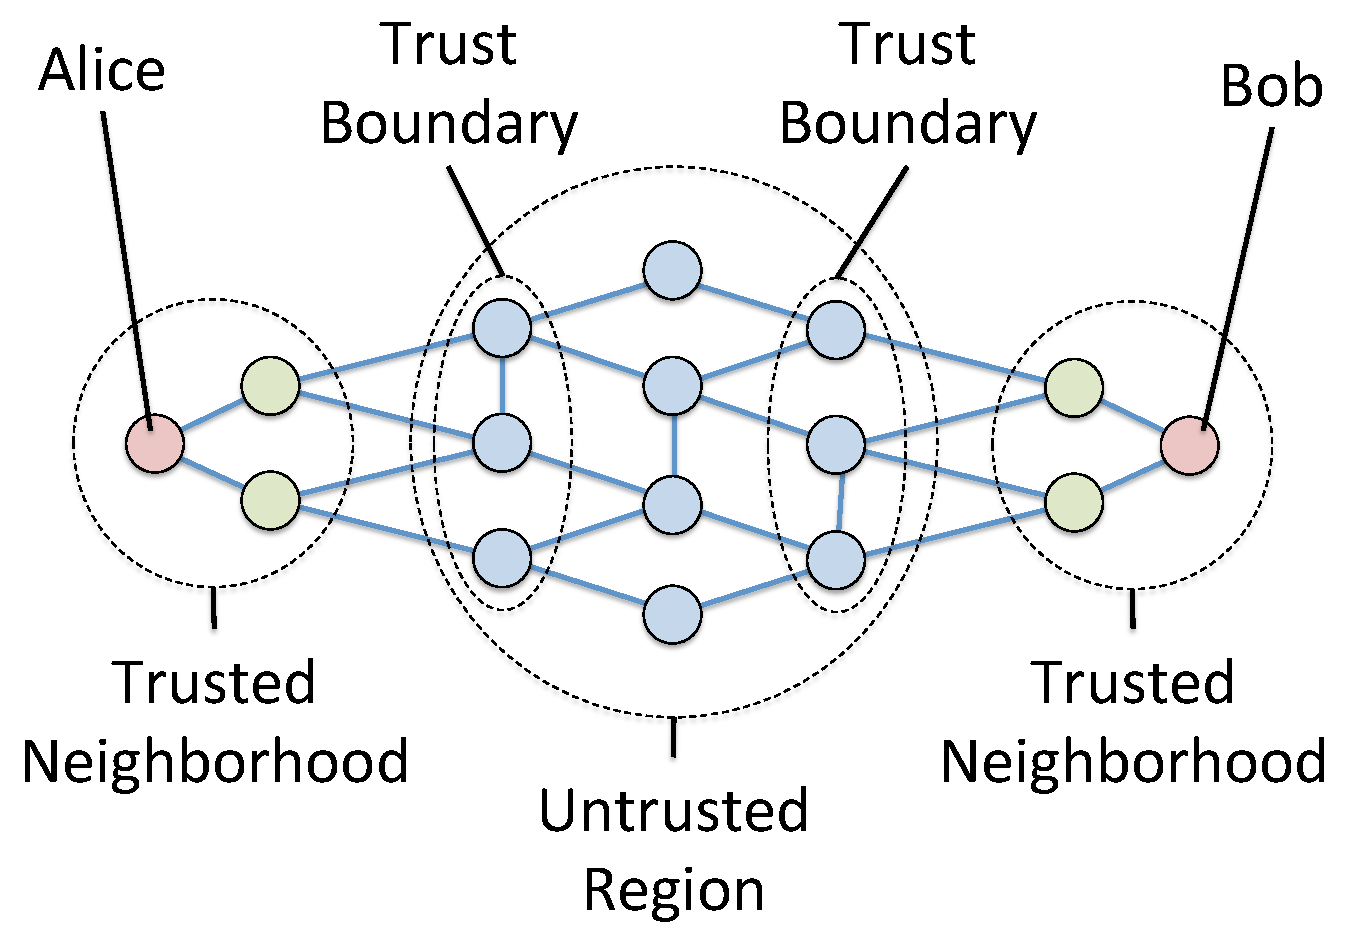
\includegraphics[width=3in,height=2.08in]{fig-partial-trust}}
\caption{
Illustration of a trusted communication network and the network properties
used by the {\em partial trust model}.
Edges represent mutually trusted communication links.
The sender (Alice, $v$) and receiver (Bob, $w$) trust all nodes
less than the {\em trust radius} $h$ hops away.
These nodes form their {\em trusted neighborhoods} $T_h(v)$ and $T_h(w)$.
We assume that all faults occur in the remaining nodes: the
{\em untrusted region}.
The untrusted nodes in contact with the trusted neighborhoods for the
{\em trust boundaries} $B_h(v)$ and $B_h(w)$,
which (in the absence of central bottlenecks) determine the
{\em effective redundancy} $\delta_h$ provided by the network.
Alice and Bob can be modelled as connected by a direct link with
at least $\delta_h$ redundant channels.
}
\label{fig:trust-source}
\end{figure}

\subsection{Multipath Fault Tolerance}

Once we have determined a network's effective redundancy,
we can apply redundancy-based fault tolerance techniques,
by sending multiple copies of a message
({\em concurrent multipath routing}).
We model our sender (Alice) and receiver (Bob) as
communicating over a direct link with $\delta_h$ redundant channels.
The partial trust model allows us to make this simplifying assumption
for analyzing a fault tolerance scheme,
but implementing such a scheme will require a method for constructing
specific network paths.
We will return to the question of constructing paths in the next section.
For now, we concern ourselves with the question:
given that the network provides $\delta_h$ redundant channels between
Alice and Bob,
what is the probability that an adversary (Mal) causes an undetectable
error?

Let us first assume that Alice sends a message copy over each available
channel.
When Bob receives the messages, there are several possibilities.
If some of the messages are missing
(Alice can include the number of messages as part of the message)
or if some of the messages disagree,
Bob knows that some of the messages were either blocked or altered,
and he has successfully detected an error.
Bob has not accepted any compromised information,
and can request retransmission, so no failure has occurred.
If Bob receives all of the messages, and they all agree,
he accepts the message.
If the messages agree, there are two possible cases.
The first case is that Mal has not compromised any of the messages,
and Bob has correctly accepted them, so no failure has occurred.
The second case is that Mal has compromised {\em all} of the messages,
so Bob has accepted an erroneous message and a failure has occurred.
In the present scenario,
whether this occurs depends only on whether Mal has the resources to
compromise all of the channels.
In a more realistic, and more interesting, scenario,
both Alice and Mal have limited resources and are not able to use or
compromise all available channels.

In a more sophisticated multipath fault tolerance scheme,
Alice randomly chooses $k \leq \delta_h$ channels and sends a copy of
her message on each.
We assume that Mal is capable of compromising $l \leq \delta_h$ channels.
Having full knowledge of the network,
Mal's best strategy is to identify a minimum node cut in the network
and compromise nodes from that cut.
With this strategy, each compromised node reduces effective redundancy by one,
effectively compromising one of the virtual channels between Alice and Bob.
Since Alice chooses channels randomly,
all channels are equally likely to contain a message,
so Mal can do no better than also choosing randomly.
If $k > l$, at least one message will get through uncompromised and all
errors are detectable.
Otherwise, the probability of Mal producing an undetectable error is
the probability that all of Alice's chosen channels are compromised:
\beq
\label{eq:pf}
p_f &=& \frac{l!(\delta_h-k)!}{\delta_h!(l-k)!}.
\eeq
Letting $k=\alpha \delta_h$ and $l=\beta \delta_h$, then applying Stirling's
approximation gives:
\begin{eqnarray}
\label{eq:pf_approx}
p_f &\approx&
\frac{\sqrt{\beta(1-\alpha)}}{\sqrt{\beta-\alpha}}
\left[
    \left( \frac{\beta-\alpha}{1-\alpha} \right)^{\alpha}
    \left( \frac{\beta}{\beta-\alpha} \right)^{\beta}
    (1-\alpha)
\right]^{\delta_h}.
\end{eqnarray}

Figure \ref{fig:pfail} shows the value of $p_f$
as a function of $k$ and $l$.
Equation (\ref{eq:pf_approx}) shows that while $p_f$
depends on the fractions of
redundant paths actually utilized $\alpha$ and compromised $\beta$,
it decreases exponentially with the effective redundancy $\delta_h$.
This result is significant because $\delta_h$
depends only on the network structure
and the strength of trust transitivity,
not on the amount of resources available to the sender or the adversary.
In other words, this scheme exhibits a {\em stabilizing asymmetry},
senders can tolerate attacks from significantly more powerful
adversaries, as long as the network structure provides large $\delta_h$.
By putting attackers at a disadvantage, attacks are not only tolerated
but also disincentivized,
further decreasing the likelihood of a successful attack.

In order to derive the above results, we have assumed that Alice and all
intermediary agents are able to identify specific,
independent network paths that achieve the effective redundancy $\delta_h$.
We now proceed to describe a routing algorithm for doing so in the special case
of the butterfly network topology.

\begin{figure}
\centerline{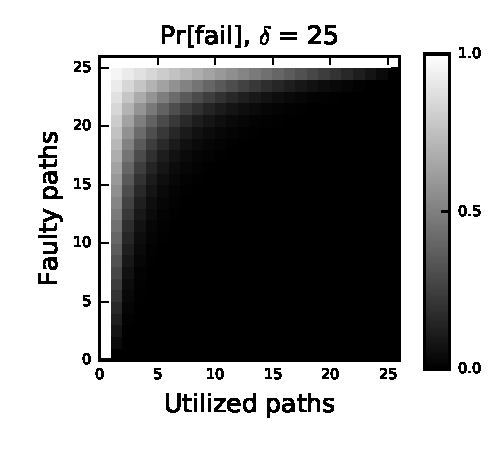
\includegraphics{fig-perror}}
\caption{
The probability of an undetectable error as a function of the number of
message copies and the number of adversarial faults.
}
\label{fig:pfail}
\end{figure}

\section{Multipath Butterfly Routing}

In previous sections, we showed that reliable communication across a network
can be achieved even when any single message path might be compromised by
an adversary,
provided the network has sufficient redundancy,
and provided the sender and intermediaries know how to route message
copies along independent paths.
In this section, we address the both requirements by proposing a novel routing
algorithm for constructing independent paths on the butterfly network topology.
This architecture and routing algorithm achieve an
effective redundancy that increases exponentially with the trust radius,
allowing a very high level of adversarial fault tolerance.

The structure of the butterfly network is highly constrained,
making it most suitable for applications where network structure can be
designed or dictated.
Examples of such networks include:
overlay networks \cite{lua_survey_2005, korzun_structured_2013},
formal organizations \cite{mohr_explaining_1982},
government-regulated cellular networks \cite{walker_mass_2012},
and call tree notification systems \cite{nickerson_thinking_2010}.
For critical security applications in particular,
the novel level of adversarial fault-tolerance offered by this scheme
is highly desirable,
even if it requires new approaches to designing communication
and trust networks.
Lastly, we note that the partial trust model and multipath fault tolerance
schemes of the previous section do not rely on any particular network
topology or routing algorithm,
and are not necessarily limited to such applications.

\subsection{Butterfly Network Topology}

We choose the butterfly topology
\cite{kshemkalyani_distributed_2008}
because of several desirable properties (described below)
and because its structure allows for relatively straightforward
design and analysis of routing algorithms.
While several variations on the butterfly network exist,
we utilize the wrap-around butterfly.
We denote the $m$-dimensional, directed wrap-around butterfly as a
graph $\wbf(m)$:
\beq
\wbf(m) &=& (V, E_\downarrow \cup E_\rightarrow) \\
V &=& \mathbb{Z}_{m} \times \mathbb{Z}_2^m \\
E_\downarrow
&=&
\{((l,z),(l+1 \; (\text{mod } m),z) \} \\
E_\rightarrow
&=&
\{(l,z),(l+1 \; (\text{mod } m),
z \oplus 1_l \},
\eeq
where $\mathbb{Z}_m$ is the set of integers modulo $m$,
$\oplus$ represents componentwise addition modulo 2,
and $1_l$ is a vector with a 1 in index $l$ and 0 elsewhere.
Each node is associated with a level $l$ and an $m$-bit string $z$
known as {\em the place-within-level}.
There are two types of edges (shown in Figure \ref{fig:butterfly}).
Down edges ($E_\downarrow$) connect nodes sharing the same $z$ value
in a cycle of increasing level $l$.
Down-right edges ($E_\rightarrow$) also link to a node of level $l + 1$,
but one having the place-within-level equal to $z$ with the $l$th bit inverted.

The wrap-around butterfly network is known to have several of the properties
we desire for scalable, decentralized communication networks:
\begin{description}
\item[Vertex-transitivity:]
Because the wraparound butterfly is vertex transitive,
it is maximally decentralized;
\item[Small-diameter:]
For any two nodes, the length of the shortest path between them is
$O(\log N)$, where N is the number of nodes in the network;
\item[Sparsity:]
With a constant degree of 4, the wraparound butterfly is extremely sparse,
and can scale indefinitely without node degree becoming a limitation;
\item [Redundancy:]
Multiple paths exist between any two nodes.
Specifically, we will prove below that the number of independent paths between two
nodes increases exponentially with the trust
radius $h$.
\end{description}

\begin{figure}
\begin{center}
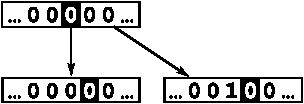
\includegraphics{fig-butterfly.pdf}
\end{center}
\caption{
Schematic illustration of the two types of edges in a directed butterfly
network.
The node $(l,z)$ is shown as the bit string $z$ with a square around the
$l$th bit.
``Down'' edges increment $l$, leaving $z$ unchanged,
while ``down-right'' edges increment $l$ and invert the $l$th bit of $z$.
\label{fig:butterfly}
}
\end{figure}

The structure of the butterfly network lends itself to a well-known
(unipath) routing algorithm,
which we later extend to the multipath case.
The unipath algorithm first follows a down or down-right edge at every step,
increasing the level $l$ by 1 and cycling through the
indices of the place-within-level.
If the current node's place-within-level matches the destination node's at
index $l$,
a down edge is chosen and the place-within-level does not change.
Otherwise, a down-right edge is chosen and the $l$th component of the
place-within-level is flipped,
after which it matches the destination.
After $m$ iterations of this, all levels have been visited
and the place-within-level matches that of the destination.
Simply following down (or up) edges will then increment (decrement) the
level until the destination node is reached.

\subsection{Multipath Routing Algorithm}

We now present a routing algorithm to construct multiple independent paths
between two nodes in a butterfly network.
Independence requires that routes between two nodes $v$ and $w$ have no nodes
in common, unless those nodes are less than distance $h$ from either $v$ or $w$.
Informally, the algorithm achieves this by using the first $h$ hops to
reach as many distinct nodes as possible,
then routing from each of those to a distinct intermediary node,
and finally routing from the intermediary to the destination.
By ensuring that the place-within-level differs for all paths
(outside of the trusted neighborhoods of $v$ and $w$)
the algorithm guaranatees independence.
As with the unipath routing algorithm,
each of the multiple paths proceed using down and down-right edges,
cycling through levels one at a time.
However, we cycle through the levels twice, once to route from $v$ to a
particular path's intermediary node,
and again to route from the intermediary to $w$.
In the first cycle, path independence is guaranteed by ensuring that
all paths differ in the first $h$ bits of the place-within-level.
Similarly, in the second cycle,
independence is guaranteed by ensuring that all paths differ in the
$h$ bits of the place-within-level preceding the destination index
(see Figure \ref{fig:route-overview}).

\afterpage{
\begin{table}[h!]
\caption{Butterfly Multipath Routing Variables\label{tab:routing}}
{
\begin{center}
\begin{tabular}{|l|l|}
\hline
NAME & VARIABLE \\\hline
butterfly dimension & $m \in \mathbb{Z}_+$ \\\hline
node level & $l \in \mathbb{Z} : 0 \leq l < m$ \\\hline
node place within level & $z \in \mathbb{Z}_2^m$ \\\hline
trust radius & $h \in \mathbb{Z} : 1 \leq h \leq \lfloor m/2 \rfloor$ \\\hline
path index & $s \in \mathbb{Z}_2^h$ \\\hline
\end{tabular}
\end{center}
}
\end{table}

\begin{figure}[t!]
\begin{center}
\begin{tikzpicture}[
node distance=0pt,
 start chain = A going right,
    X/.style = {rectangle, draw,% styles of nodes in string (chain)
                minimum width=10ex, minimum height=3ex,
                outer sep=0pt, on chain},
                        ]
\foreach \i in {0\ldots,{\ldots}0\ldots,{\ldots}0\ldots,{\ldots}0}% <-- content of nodes
    \node[X] {\i};
\draw[<->] ([yshift=1.5mm] A-1.north east) -- node[above=0.25mm] {$h$} ([yshift=1.5mm] A-1.north west);
\draw[<->] ([yshift=1.5mm] A-2.north east) -- node[above=0.25mm] {$l_w - 2h$} ([yshift=1.5mm] A-2.north west);
\draw[<->] ([yshift=1.5mm] A-3.north east) -- node[above=0.25mm] {$h$} ([yshift=1.5mm] A-3.north west);
\draw[<->] ([yshift=1.5mm] A-4.north east) -- node[above=0.25mm] {$m - l_w$} ([yshift=1.5mm] A-4.north west);
\draw ( A-1.west) -- node[left=5ex,minimum width=10ex] {start} ( A-1.west);
\node (B1) [inner sep=1pt,above=of A-1.north,above=5ex] {\underline{A}};
\node (B2) [inner sep=1pt,above=of A-2.north,above=5ex] {\underline{B}};
\node (B3) [inner sep=1pt,above=of A-3.north,above=5ex] {\underline{C}};
\node (B4) [inner sep=1pt,above=of A-4.north,above=5ex] {\underline{D}};
\end{tikzpicture}
\\
\begin{tikzpicture}[
node distance=0pt,
 start chain = A going right,
    X/.style = {rectangle, draw,% styles of nodes in string (chain)
                minimum width=10ex, minimum height=3ex,
                outer sep=0pt, on chain},
    Y/.style = {rectangle, draw,% styles of nodes in string (chain)
                minimum width=10ex, minimum height=3ex,
                outer sep=0pt, on chain, thick},
                        ]
\node[Y] {$s$};
\foreach \i in {{\ldots}0\ldots,{\ldots}0\ldots,{\ldots}0}% <-- content of nodes
    \node[X] {\i};
\draw ( A-1.west) -- node[left=5ex,minimum width=10ex] {1.} ( A-1.west);
\end{tikzpicture}
\\
\begin{tikzpicture}[
node distance=0pt,
 start chain = A going right,
    X/.style = {rectangle, draw,% styles of nodes in string (chain)
                minimum width=10ex, minimum height=3ex,
                outer sep=0pt, on chain},
    Y/.style = {rectangle, draw,% styles of nodes in string (chain)
                minimum width=10ex, minimum height=3ex,
                outer sep=0pt, on chain, thick},
                        ]
\foreach \i in {$s$}% <-- content of nodes
    \node[X] {\i};
\node[Y] {{\ldots}1\ldots};
\foreach \i in {{\ldots}0\ldots,{\ldots}0}% <-- content of nodes
    \node[X] {\i};
\draw ( A-1.west) -- node[left=5ex,minimum width=10ex] {2.} ( A-1.west);
\end{tikzpicture}
\\
\begin{tikzpicture}[
node distance=0pt,
 start chain = A going right,
    X/.style = {rectangle, draw,% styles of nodes in string (chain)
                minimum width=10ex, minimum height=3ex,
                outer sep=0pt, on chain},
    Y/.style = {rectangle, draw,% styles of nodes in string (chain)
                minimum width=10ex, minimum height=3ex,
                outer sep=0pt, on chain, thick},
                        ]
\foreach \i in {$s$,{\ldots}1\ldots}% <-- content of nodes
    \node[X] {\i};
\node[Y] {$\tilde{s}$};
\foreach \i in {{\ldots}0}% <-- content of nodes
    \node[X] {\i};
\draw ( A-1.west) -- node[left=5ex,minimum width=10ex] {3.} ( A-1.west);
\end{tikzpicture}
\\
\begin{tikzpicture}[
node distance=0pt,
 start chain = A going right,
    X/.style = {anchor=base, rectangle, draw,% styles of nodes in string (chain)
                minimum width=10ex, minimum height=3ex,
                outer sep=0pt, on chain},
    Y/.style = {rectangle, draw,% styles of nodes in string (chain)
                minimum width=10ex, minimum height=3ex,
                outer sep=0pt, on chain, thick},
                        ]
\foreach \i in {$s$,{\ldots}1\ldots,$\tilde{s}$}% <-- content of nodes
    \node[X] {\i};
\node[Y] {$z_{w,D}$};
\draw ( A-1.west) -- node[left=5ex,minimum width=10ex] {4.} ( A-1.west);
\end{tikzpicture}
\\
\begin{tikzpicture}[
node distance=0pt,
 start chain = A going right,
    X/.style = {anchor=base, rectangle, draw,% styles of nodes in string (chain)
                minimum width=10ex, minimum height=3ex,
                outer sep=0pt, on chain},
    Y/.style = {rectangle, draw,% styles of nodes in string (chain)
                minimum width=10ex, minimum height=3ex,
                outer sep=0pt, on chain, thick},
                        ]
\node[Y] {$z_{w,A}$};
\foreach \i in {{\ldots}1\ldots,$\tilde{s}$,$z_{w,D}$}% <-- content of nodes
    \node[X] {\i};
\draw ( A-1.west) -- node[left=5ex,minimum width=10ex] {5.} ( A-1.west);
\end{tikzpicture}
\\
\begin{tikzpicture}[
node distance=0pt,
 start chain = A going right,
    X/.style = {anchor=base, rectangle, draw,% styles of nodes in string (chain)
                minimum width=10ex, minimum height=3ex,
                outer sep=0pt, on chain},
    Y/.style = {rectangle, draw,% styles of nodes in string (chain)
                minimum width=10ex, minimum height=3ex,
                outer sep=0pt, on chain, thick},
                        ]
\foreach \i in {$z_{w,A}$}% <-- content of nodes
    \node[X] {\i};
\node[Y] {$z_{w,B}$};
\foreach \i in {$\tilde{s}$,$z_{w,D}$}% <-- content of nodes
    \node[X] {\i};
\draw ( A-1.west) -- node[left=5ex,minimum width=10ex] {6.} ( A-1.west);
\end{tikzpicture}
\\
\begin{tikzpicture}[
node distance=0pt,
 start chain = A going right,
    X/.style = {anchor=base, rectangle, draw,% styles of nodes in string (chain)
                minimum width=10ex, minimum height=3ex,
                outer sep=0pt, on chain},
    Y/.style = {rectangle, draw,% styles of nodes in string (chain)
                minimum width=10ex, minimum height=3ex,
                outer sep=0pt, on chain, thick},
                        ]
\foreach \i in {$z_{w,A}$,$z_{w,B}$}% <-- content of nodes
    \node[X] {\i};
\node[Y] {$z_{w,C}$};
\foreach \i in {$z_{w,D}$}% <-- content of nodes
    \node[X] {\i};
\draw ( A-1.west) -- node[left=5ex,minimum width=10ex] {7.} ( A-1.west);
\end{tikzpicture}
\end{center}
\caption{
Progression of place-within-level $z$ as the multipath routing algorithm
cycles through the levels of the butterfly network.
\label{fig:route-overview}
}
\begin{center}
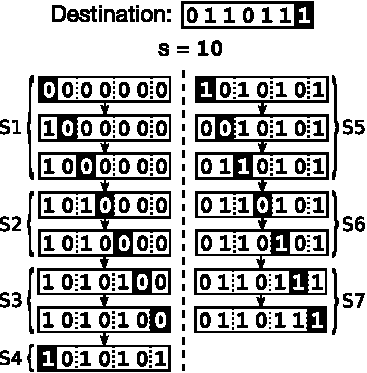
\includegraphics{fig-routing.pdf}
\end{center}
\caption{
An example of one path as constructed by the proposed multipath
routing algorithm.
The path is shown for $s = 10_2$
and $w = (6, 0110111_2)$.
\label{fig:routing}
}
\end{figure}
}

We now begin the formal specification of our multipath routing scheme for the
wraparound butterfly network.
Utilizing vertex transitivity, we label the source node as
$(l^{(0)}, z^{(0)}) = (0, 0)$ and denote the destination node as $w = (l_w, z_w)$,
without loss of generality.

Let $s$ be an $h$-bit binary string with $s_i$ denoting the bit at index $i$.
There are $2^h$ such strings.
Let $v_s^{(t)} = (l^{(t)}, z^{(t)})$ be the node at position $t$
in the path parameterized by $s$.
For convenience,
we will omit the subscript $s$ when it is obvious from context.
We define three distinct partitions of $m$-bit binary strings.
Let $Q_{v^{(0)}}$ ($\overline{Q_{v^{(0)}}}$) be the set of $m$-bit
strings in which the bits at
all indices $h \leq i < l_w - h$ match (do not all match) those of $z^{(0)}$.
Note that $Q_{v^{(0)}}$ is trivially all $m$-bit strings if $l_w < 2h$.
Let $R_s$ ($\overline{R_s}$) be the set of $m$-bit strings with the lowest $h$
bits all matching (not all matching) the bits of $s$.
Let $S_s$ ($\overline{S_s}$) be the set of $m$-bit strings with the $h$ bits
preceding index $l_w$ all matching (not all matching) the bits of $\tilde{s}$,
where $\tilde{s}$ is a cyclic permutation of $s$:
\beq
\tilde{s}_i &=& s_{(i + l_w) \text{ mod } h}.
\eeq
We will make use of the fact that:
\beq
s \neq s^\prime &\implies&
S_s \cap S_{s^\prime} = R_s \cap R_{s^\prime} = \emptyset.
\eeq

Routes are constructed in 7 stages.
The network topology dictates that $l^{(t+1)} = l^{(t)} + 1$ (mod $m$),
so we let $l = t$ (mod $m$).
and that $z^{(t+1)}$ is equal to $z^{(t)}$ with or without the bit in index
$l^{(t)}$ inverted, depending on whether the down or down-right edge was
taken at step $t$.
\begin{description}
\item[Stage 1: ($0 \leq t < h$)]{
Down or down-right edges
are chosen such that the $t$th bit of $z^{(t+1)}$ is equal to the $t$th bit
of $s$.
Throughout Stage 1, all nodes are within the sender's trusted neighborhood.
Throughout Stage 1, $z^{(t)} \in Q_{v^{(0)}}$.
At the end of Stage 1, $z^{(h)} \in S_s$, and $z^{(t)}$ will remain so until the level cycles to $0$ at $t = m$.
}
\item[Stage 2: ($h \leq t < l_w - h$)]{
Edges are chosen to make the $t$th bit of
$z^{(t+1)}$ the inverse of the $t$th bit of $z^{(0)}$.
Note that this stage does not occur when $l_w < 2h$.
If this stage occurs, then $z^{(t)} \in \overline{Q_{v^{(0)}}}$ until these
levels are reached again in stage 6.
}
\item[Stage 3: ($l_w - h \leq t < l_w$)]{
The bits of $z^{(t)}$ are chosen to match $\tilde{s}$,
such that after the stage is complete, $z^{(t)} \in R_s$.
}
\item[Stage 4: ($l_w \leq t < m$)]{
Paths are chosen such that the $t$th bit of $z^{(t+1)}$ matches that of the
destination node $z_w$.
This stage will not occur if $l_w > m - h$.
}
\item[Stage 5: ($m \leq t < m + h$)]{
There are two cases.
If $2h < l_w < m - h$,
then there is no overlap between the indices defining $R_s$ and $S_s$.
In this case, the first $h$ bits of $z^{(t)}$ are set to
match $z_w$.
Otherwise there is some overlap between the indices defining $R_s$ and
$S_s$.
In this case, the each of the first $h$ bits of $z^{(t)}$ is either kept the
same if $l_w - h \leq l < l_w$, or set to the corresponding bit of $z_w$
otherwise.
In this stage and after, $z^{(t)}$ is no longer guaranteed to be in $R_s$.
However, $z^{(t)}$ remains in $S_s$ during and after this stage.
}
\item[Stage 6: ($m + h \leq t < m + l_w - h$)]{
In this stage, edges are chosen to set the bits of $z^{(t)}$ to their
corresponding value in $z_w$.
$z^{(t)} \in \overline{Q_{v^{(0)}}}$ throughout this stage,
but not afterwards.
}
\item[Stage 7: ($m + l_w - h \leq t < m + l_w$)] {
The $h$ bits of $z^{(t)}$
preceding index $l_w$ are set to match $z_w$.
All nodes in this stage are within $h$ hops of $w$ and thus in its trusted
neighborhood.
After this stage, $v^{(m + l_w)} = w$ and routing is complete.
}
\end{description}

\begin{theorem}
Given an $m$-bit wraparound butterfly network ($m \geq 0$),
and a trust radius $h \geq 1$,
for all node pairs $(v, w)$,
if there exists a node $u$ that belongs to
two distinct routes $v^{(\cdot)}_s$ and $v^{(\cdot)}_{s^\prime}$
($s \neq s^\prime$),
it implies that $u \in T_h(v) \cup T_h(w)$.
\end{theorem}
\begin{proof}
Nodes from two paths can only coincide if their levels are the same.
Nodes which share a level must either be in the same stage, or 4 stages
apart.
Let ($a$,$a^\prime$) denote a pair of sub-paths corresponding to stage $a$ of
one path and stage $a^\prime$ of another.
Excluding paths that intersect in their trusted neighborhoods, (1,1) and (7,7),
we have reduced the list of possible intersections to the following cases:
(2,2), (3,3), (4,4), (5,5), (6,6), (1,5), (2,6), and (3,7).
Nodes in stages 2--4 belong to $R_s$ so cannot overlap with any stage 2--4
nodes from another path, eliminating (2,2), (3,3), and (4,4).
Similarly, nodes in stages 4--6 belong to a unique $S_s$,
eliminating (5,5) and (6,6).
Nodes in stage 1 belong to $Q_{v^{(0)}}$ while those in stage 5 belong in
its complement, eliminating (1,5).
Similarly, for all $l$ in stage 2, $z^{(l)}$ is equal to $z^{(0)}$,
while in stage 6, $z^{(l)}$ is the inverse, eliminating (2,6)
This leaves only (3,7), a collision which can occur only for only one path
(with $s$ matching the first $h$ bits of $z_w$), and which enters the trusted
neighborhood in stage 3.
For this single path, we can proceed directly from stage 2 to stage 7,
eliminating the last possible collision.
\end{proof}

Thus, assuming the partial trust model with trust transitive
for $h$ hops, we can construct $2^h$ paths on a wraparound butterfly topology
which do not intersect outside the trusted neighborhoods of the source and
destination.
Note that the node sequence $v_s^{(t)}$ can be calculated entirely
from the source $v$, destination $w$, and path parameter $s$,
meaning that with this information nodes are able to determine which neighbor
to route a given message copy to.
Furthermore, the existence of $2^h$ paths places a lower bound on the
effective redundancy $\delta_h$,
showing that the decentralized, redundant, structured networks such as the
butterfly can have a very low probability of failure when faced with
adversarial faults, even from a very powerful attacker.

\section{Discussion}

While decentralized protocols have received much attention for their potential
fault tolerance applications,
a better understanding of how network structure contributes to fault tolerance
is necessary.
We have proposed a number of contributions towards this understanding:
a {\em partial trust model} for quantifying the effective redundancy
of a network,
a {\em multipath fault tolerance} scheme for using that redundancy to detect
errors,
and a {\em concurrent multipath routing} algorithm enabling this scheme to
be implemented on the butterfly network.

Fault-tolerant network infrastructures have many direct applications.
Areas such as cryptocurrency
\cite{mazieres_stellar_2015,nakamoto_bitcoin:_2008,king_ppcoin:_2012},
secure multiparty computation
\cite{yao_protocols_1982,chaum_multiparty_1988,goldreich_how_1987},
and wireless sensor networks
\cite{khiani_comparative_2013}
have immediate need for scalable, fault-tolerant infrastructures.
Many Internet services (e.g., email, social networks, cloud storage)
are still highly centralized and vulnerable to technical and
non-technical (i.e. coercive) attacks.
Fault tolerance using {\em both} decentralized protocols and
decentralized network structures
is one approach to securing these important
services and making networked communication safer.

We have also focused specifically on adversarial faults that block or
change messages (e.g., censorship).
We have not specifically addressed {\em confidentiality}:
how to keep those messages private.
Existing cryptographic techniques for confidentiality are relatively
mature compared to those for tolerating censorship.
In fact, an attacker might use targeted attacks to achieve censorship
as a fallback when surveillance isn't feasible.
However, the techniques presented in this paper
are entirely compatible with, and in some cases could enhance, existing
confidentiality techniques.
For example, the well-known {\em man-in-the-middle} attack exploits a privileged
network position to attack otherwise secure cryptography,
suggesting that structural approaches can complement cryptographic ones.

Our multipath fault tolerance scheme can be applied to any network
that has both sufficient redundancy and a routing algorithm
that maps local links to independent network paths.
These requirements make the approach well-suited for structured networks,
in which link structure can be dictated,
such as the butterfly.
While the ability to control network topology is only achievable in some
applications, those applications are nonetheless significant
(e.g. overlay networks \cite{lua_survey_2005, korzun_structured_2013},
formal organizations \cite{mohr_explaining_1982},
government-regulated cellular networks \cite{walker_mass_2012},
and call tree notification systems \cite{nickerson_thinking_2010}).
Furthermore, when high levels of adversarial fault tolerance are required,
new sociotechnical systems might choose to incorporate such networks.
For example,
a coalition of groups supporting free expression could use our results
to construct a censorship-resistant communication network
by cultivating the necessary trust relationships.
In the general case,
while the partial trust model can be applied to unstructured networks,
additional work is needed to identify how to ensure redundancy and
identify independent paths in unstructured networks.

\section{Conclusion}

We have developed a partial trust model which enables a formal analysis
of the effect of network structure and trust transitivity on
redundancy.
We have also proposed a multipath fault tolerance scheme
for using this redundancy to achieve adversarial
fault tolerance.
Under this scheme, the probability of an adversary causing an undetectable error
decreases exponentially with the network's effective redundancy.
Furthermore, a small increase in the number of messages sent can compensate
for a large increase in the number of messages compromised by an adversary.
This stabilizing asymmetry puts attackers at a disadvantage,
disincentivizing attack.
We also presented a novel multipath routing algorithm allowing multipath fault
tolerance to be used on the butterfly topology,
and proved that the effective redundancy of the butterfly network increases
exponentially with the trust radius.
These results are directly applicable to architectures in which the link
structure can be imposed by the architect,
and more generally, provide a formalism that can be used more to evaluate
the role of network structure, trust transitivity, and effective redundancy
on adversarial fault tolerance.

%ACKNOWLEDGMENTS are optional
\section{Acknowledgments}
Anonymized for blind review.

%
% The following two commands are all you need in the
% initial runs of your .tex file to
% produce the bibliography for the citations in your paper.
\bibliographystyle{abbrv}
\bibliography{paper}  % sigproc.bib is the name of the Bibliography in this case
% You must have a proper ".bib" file
%  and remember to run:
% latex bibtex latex latex
% to resolve all references
%
% ACM needs 'a single self-contained file'!
%
%
\end{document}
